\documentclass[hidelinks,12pt]{article}
\linespread{1.3}
\usepackage{hyperref}
\usepackage{enumerate,changepage,lipsum,titlesec, longtable}
\usepackage{cite}
\usepackage{comment, xcolor}
\usepackage[pdftex]{graphicx}
  \graphicspath{{images/}, {images/stat/}}
  \DeclareGraphicsExtensions{.pdf,.jpeg,.png, .jpg}
\usepackage[cmex10]{amsmath}
\usepackage{array} 
\usepackage{subfigure} 
\newcommand{\grey}[1]{\textcolor{black!30}{#1}}
\newcommand{\red}[1]{\textcolor{red!50}{#1}}
\newcommand{\fref}[1]{Figure \ref{#1}}
\newcommand{\tref}[1]{Table \ref{#1}}

\oddsidemargin0cm
\topmargin-2cm %I recommend adding these three lines to increase the
\textwidth16.5cm %amount of usable space on the page (and save trees)
\textheight23.5cm

\makeatletter
\renewcommand\paragraph{\@startsection{paragraph}{4}{\z@}%
            {-2.5ex\@plus -1ex \@minus -.25ex}%
            {1.25ex \@plus .25ex}%
            {\normalfont\normalsize\bfseries}}
\makeatother
\setcounter{secnumdepth}{4} % how many sectioning levels to assign numbers to
\setcounter{tocdepth}{4}    % how many sectioning levels to show in ToC


\begin{document}
\title{Dynamic Energy Mapping Project Outline}
\maketitle
\tableofcontents
\newpage
\section{General Introduction}
\subsection{Project Overview}
\begin{comment}
Buildings alone account for 40\% of the total energy usage in the
United States. However if the indirect energy impact of the built
environment as a whole was considered, the community design induced
energy and environmental impact could exceed this already high ratio:
60\% - 75\% of the energy consumption is connected to the spatial
layout of built environment~\cite{Owens199281}. In a broader sense,
the energy resources distribution influences the layout of human
activities~\cite{Owens199281}. In a more restrict sense, built
environment influence the community energy throughput by its density,
degree of land use mix, energy supply infrastructure and
transportation network ~\cite{Jaccard19971065}.
\end{comment}

The burning of fossil fuels produces green house gas (GHG) and causes
significant global climate changes including global sea level rise,
temperature rise, ocean warming, ice sheet melting and extreme weather
event~\cite{NASA2015}. Fossil fuels are finite: studies have shown
that if the consuming rate of fossil fuels remain the same, the major
fossil fuels including oil, gas and coal will run out by the end of
the century~\cite{Ecotricity2015, Kathryn2015}. Governments began to
put reducing GHG as one of their major goals: the ``Climate Change
Act'' of UK aims at reducing GHG emissions by 80\% comparing to 1990
by 2050~\cite{carbonBudgetUK}, the City of Calgary aims at reducing
CO$_2$ emission rate by 50\% by 2050~\cite{aacip2009}. 

Reducing GHG emission and fossil fuel consumption also took place on
the community level. Community Energy Management (CEM) is a
combination of community level design strategies and energy management
strategies aiming at providing quality of life in an urban environment
with minimized energy consumption and environmental
impact~\cite{Jaccard19971065}. It contains ``land use planning'',
``transportation management'', ``site planning'' and ``local energy
supply and delivery planning''~\cite{Jaccard19971065}. Community level
energy planning and management achieves GHG reduction by means of :1)
improving energy usage efficiency, 2) conserving the use of high
quality energy and 3) switching to using more renewable energy source
~\cite{StDenis20092088}. 

Energy Mapping makes the community energy planning alternatives
visible to planners and policy makers~\cite{baird2014} and thus
flourishes under this trend. Emerging explorations on the
functionality and the power of Energy Mapping in assisting community
energy planning are taking place all over the world. City of Calgary
carried out an Energy Mapping Study that aims to ``provide clear
direction to the City and inform the private sector about the
potential to reduce greenhouse gas emissions and encourage the use of
alternative energy systems, through considerations such as the design
of buildings and encouragement of more compact, mixed-use and high
density communities.''~\cite{baird2014}.  

What information should an Energy Map hold and in what form should the
information be conveyed or displayed is still not completely agreed
between different approaches. Calgary Energy Mapping study depicts
annual average energy use intensity and alternative renewable energy
supply region~\cite{aacip2009}. London Heat Map contains mainly
heating energy related features: high heating energy consumers,
suppliers and district heating networks. Dutch Heat Map, an
application of the EPM method, contains information of annual heating
energy demand (or demand density), heating energy supply (or supply
density), infrastructure network layout and CHP and Biomass plant
location.

However, as suggested by Baird et al.\ existing Energy Mapping
practices are mainly static, i.e. the time-dependent changes of energy
demand and supply information is not included in these Energy Maps nor
do they support more advanced community energy system analysis and
comparison. Thus the concept of ``Dynamic Energy Map'' was brought
about: It acts as a geo-database that holds 1) hourly energy profile
data for each building and the aggregated energy profile data for the
whole community; 2) hourly energy supply data of community
decentralized energy sources~\cite{baird2014}. 

With the Dynamic Energy Map, the temporal behavior of the demand and
supply of heating, cooling and electricity are revealed and are
available to be compared, analyzed and updated. For example, the
Dynamic Energy Map will show the spatial and temporal changes of peak
energy demand and supply and verifies whether and how well the supply
meets the demand over time. A Dynamic Energy Map is also connected to
simulation software~\cite{baird2014}, and can act as a key component
of Geo-design that encompasses ``geo-spatial modeling, impact
simulations, and real-time feedback to facilitate holistic designs and
smart decisions''~\cite{esriGeodesign2012}. The development of
data-driven approaches and machine learning methods could also be
coupled and can perform more complicated analysis of spatial-temporal
behavior of energy data and provide more informative design or
management support.

An initial instance of Dynamic Energy Map was created by Baird et al.\
in 2011-2012. The map consists of two parts: a geo-database that holds
general building information (name, conditioned area) annual and
monthly energy usage information (energy use intensity, annual peak
demand value and monthly peak demand value); an excel screening tool
that holds hourly energy usage information of each building and
performs analysis and system comparison of a district energy
system~\cite{baird2014}.

\subsection{Objective and Problem Definition}
Appealing to the definition of Dynamic Energy Map~\cite{baird2014},
its major functions could be summarized as: 1) holding, 2) visualizing
and 3) analyzing community level high spatial-temporal resolution
energy demand and supply data 4) connection to simulation engine for
iterative performance analysis. In the initial instance of Dynamic
Energy Map by Baird et al.\ ~\cite{baird2014}, function 1) of holding
spatial-temporal (although with low temporal resolution) energy data
is realized. Function 4) of connecting to building simulation data is
also realized by importing simulation result csv files to the
geo-database (although with low temporal resolution). Function 2)
visualizing and 3) analyzing high resolution energy data remains to be
done.

For function 3), although the geo-database and the analysis is
conducted separately, it is possible to export the analysis result and
aggregate it to the geo-database. For function 2), the spatial and
temporal information are visualized separately: the spatial
information of 3D building geometry and location could be visually
inspected in the geo-database but not the hourly energy consumption
information. 2) The temporal visualization of energy demand is done
separately in the excel screening tool as 3D graphs, but no spatial
context is present and the spatial dimension is then lost. The authors
thus identified the crucially missing function: the visualization of
such a spatial-temporal changing of energy behavior as the major goal
of the current project.

The objective of the project is thus defined as to 1) implement a
Dynamic Energy Demand Map with the focus on creating a high-resolution
spatial-temporal visualization of hourly thermal energy consumption
data for each building, major building sectors and the whole community
2) testify the its use in optimizing the arrangement of land use
pattern to improve the community level energy performance in terms of
aggregated thermal energy demand variation and 3) support sizing of a
district thermal energy supply system.

The community model is created in City Engine~\cite{cityEngine2015}
based on the land use pattern of a mixed-use redevelopment project at
Lower Hill District, Pittsburgh, PA~\cite{Ramesh2013}. The model
contains 68 buildings, comparable to a typical service area of a
district thermal energy system (combined heating and cooling), about
50 to 150 buildings~\cite{IDEA2005}.

The hourly heating (gas) and cooling energy (electricity) consumption
profile is retrieved from DOE Commercial Benchmark Building
simulation~\cite{DOE2015}. An interface was designed to combine the
8760 heating-cooling energy choropleth map images from City Engine and
the 8760 hourly heating-cooling energy data from EnergyPlus to form a
Dynamic Energy Map. The interface provides users with the functions of
1) navigating through the dynamic map images, 2) dynamic data
plots of single buildings, building sectors and aggregated community
thermal energy demand.

\subsection{Related Concepts}\label{concept}
Some related key concepts will be discussed in this section: the
district energy system, the Energy Map and the Dynamic Energy Map.

\subsubsection{District Energy System}
A district energy system is one form of Decentralized Energy System, a
``local or sub-regional supply of energy from a local
source.''~\cite{lhmreport2012}. It brings the energy generation near
to the energy end users and reduces the energy transmission and
distribution loss~\cite{decentralHeatMap2011}.

A district energy system produces thermal energy in a central plant
and deliver the thermal energy to local buildings through a
closed-loop pipeline network. Thermal energy are delivered in the form
of steam, hot water or chilled water~\cite{baird2014}. The central
power plant can take on one of the following forms: 1) thermal power
plant that only generates thermal energy, which can be either heating
or cooling energy 2) co-generation system, or combined heat and power
(CHP) system, that generates electricity and reuses the reject heat
from electricity generation to serve space heating and service hot
water to local buildings~\cite{IDEA2005} 3) tri-generation system,
where the central plant uses the heat generated by CHP plant to
produce chilled water and supply both heating and cooling energy
~\cite{cchp2015}. Corresponding to the different types of power plant,
the network delivering thermal energy can be classified as 1) district
heating network that only delivers steam or hot water 2) district
thermal network that delivers both heating energy in the form of steam
or hot water and cooling energy as chilled water.

A district thermal energy system corresponds to the three means of GHG
reduction as follows:
\begin{itemize}
\item High energy generation efficiency

  Higher energy usage efficiency means with the same amount of input
  energy, more useful energy is produced and less are
  wasted. Buildings' electricity supply are mainly from centralized
  power plant that are far away from cities. Heat produced in power
  generation are normally dumped into oceans and
  lakes~\cite{baird2014, IDEA2012}, not only causing negative
  environment impact~\cite{wasteHeatEnviron}, but also reduce the
  power generation efficiency to be only about
  1/3~\cite{IDEA2012}. District Energy System has high energy
  generation efficiency as a result of 1) it can utilize high
  efficiency large-scale energy generation equipment~\cite{IDEA2005}
  and 2) it is closer to the energy end user which reduces the energy
  loss due to transmission and distribution~\cite{IDEA2012}.

\item Better Exergy Performance 

  The quality of energy is usually described with exergy. It is
  defined as ``maximum useful work possible during a process that
  brings the system into equilibrium with a heat
  reservoir''~\cite{exergyWiki2015}. It represents the energy one can
  get out of the system. One example of a District Energy system helps
  improving exergy performance and better match the thermal energy
  supply and the low and medium-quality building energy demand
  ~\cite{Dobbelsteen2013} is the low-temperature (or low-energy)
  district heating system~\cite{Tol2012551} which has a supply
  temperature of around 50~$^o$C and return temperature of around
  25$^o$~C~\cite{Tol2012551}.

\item Multiple fuel choices including renewable energy sources

  The central plant of a district energy system can use a broad range
  of fuel choices including natural gas, oil, coal, waste, and
  renewable energy sources including geothermal, solar thermal and
  biomass, in the generation of thermal energy. This makes the switch
  to large scale renewable energy source possible. It also makes the
  district thermal energy system more flexible and more competitive in
  the market and increases the energy system
  resilience~\cite{IDEA2005, IDEA2012}.

\end{itemize}

It also reduces the space and cost dedicated to installation and
maintenance of HVAC systems in single buildings. It also reduces
harmful gas emission of NO$_x$, SO$_x$ by using non-combustion energy
sources as lake body and by filtering~\cite{IDEA2012} the flue gas~\cite{veolia2014}.

\subsubsection{Heat Map}
Although ``heat map'' is generally accepted as ``graphical
representation of data where the individual values contained in a
matrix are represented as colors''~\cite{HeatmapWiki}, with respect to
buildings, a ``heat map'' may be defined as ``a spatial plan of
existing and planned building heat demand, and decentralized energy
networks and generation equipment''~\cite{decentralHeatMap2011}. It is
also a GIS ``live database'' that allows new development information
to be incorporated. It is a key component to the decentralized energy
master plan~\cite{decentralHeatMap2011}. One of the well-known
instances of a heat map is the ``London Heat
Map''~\cite{londonHeatMap}

\subsubsection{Energy Map}
International District Energy Association (IDEA) define Energy Map as:
``a tool that can be used to organize/present data as the basis for
defining energy character areas as part of energy
planning''~\cite{IDEA2012}. It is a ``GIS based system'' that can be
used to develop energy strategies, prioritize project, identify
potential growth opportunities and impose planning
restrictions~\cite{IDEA2012}. Dobbelsteen et al.\ adopted the term
``Energy Potential Mapping'' that assist the development and plan of a
sustainable built environment. It is a method that ``visualizes local
energy potentials and demand in order to support spatial planning
towards more energy-efficient urban or rural
environment''~\cite{Dobbelsteen2013}. UK used the ``Decentralized
Energy Masterplanning'' as a method that helps local authorities
identify low carbon strategies that ``maximises the opportunity for
large-scale schemes to capture and use waste heat from major energy
sources''~\cite{decentralHeatMap2011}.

With respects to the various definitions above, an Energy Map could be
understood as a generalization of a heat map that includes energy
supply, demand and infrastructure information of various energy forms
and technologies. Some existing use cases of suggest an Energy Map
could be used to visualize the community or city level energy demand
reduction with high performance building design~\cite{aacip2009} or
adoption of alternative energy supply
technologies~\cite{aacip2009}. It can be used in supporting district
heating system design~\cite{decentralHeatMap2011, Finney2012165} by
visualizing the heat sources and sinks.

\subsubsection{Dynamic Energy Map}
According to the study of Baird et al.\ , a Dynamic Energy Map is a
Energy Map equipped with temporal information of energy supply and
demand. It enables spatial-temporal comparison, aggregation and query
of energy demand and supply. It is coupled with Energy simulation
tools, and design alternatives would be evaluated and compared at each
given time spot or time period. By performing advanced data analysis
method, the dynamic map makes patterns that are omitted in static maps
visible and analyzable. Both aspects enable more detailed energy
analysis and design support.

\subsection{Why ``time'' dimension is important for an Energy Map}
\subsubsection{Strong Temporal Variation of Energy Demand}
Different building types often indicates different energy demand
profile. For example, the residential building heat demand profile has
two major peaks, morning and evening, and is relatively low for the
rest of the day. For office buildings, there is a peak heat demand in
the morning and a relatively high heat demand through the day time but
drops in the evening. Hospitals usually have a more flattened demand
throughout the day. Within a mixed-used urban environment, the arrival
of peak demand for different buildings are usually not
simultaneous~\cite{decentralHeatMap2011}.

In the design of a district energy system, mixing building types with
different time-of-use energy profile can be helpful in creating a less
variate aggregated energy demand. This allows the central CHP plant in
a district energy system to a have higher utilization rate and reduces
the need for backup plant that accounts for high peak
demand~\cite{decentralHeatMap2011}.

\begin{figure}[h!]
  \centering
  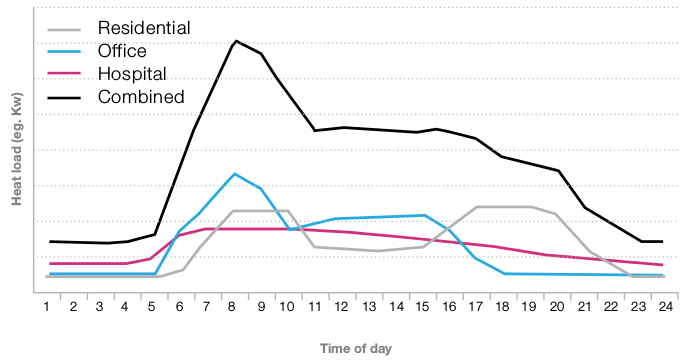
\includegraphics[width=0.7\linewidth]{mixLoad.png}
  \caption{Mixing Load of Different Building
    Type~\cite{decentralHeatMap2011}}
  \label{fig:mixLoad}
\end{figure}

\subsubsection{Aggregation of Peak Value Becomes Tricky for Data with Time Variation}
One common mistake for sizing a district thermal energy system is to
add up the peak demand of each terminal users. Since the peak demand
of individual buildings do not occur at the same time, the end result
of summing up the peak demand at each end point exceeds the actual
total demand peak of the community, hence with this approach, the
whole district system becomes excessively over-sized, which reduces
the whole system efficiency. A Dynamic Energy Map can reveal the
problem of such approaches by directly providing the aggregated
thermal energy demand for the community and for single buildings or
building sectors. It allows a side by side comparison of single
building demand and aggregated demand and eliminates the
misunderstanding of the demand aggregation. With the direct
information of aggregated thermal energy demand, it also assists
actually sizing a district thermal energy system.

\newpage
\section{Related Works}
Section \ref{staticEnergyMap} and section \ref{dynamicMap} provide an
overview of the existing instances of static energy maps and dynamic
energy maps. A list of summary of techniques used in the production of
Static and Dynamic Energy Map instances are as in
\tref{tab:mapSummary}:

\begin{comment}
Section \ref{mapDesign} and \ref{stDataAnalysis} provides
some supporting evidences for certain design choices. Section
\ref{4dMap} provides some information on potential technologies for
further development. \grey{(?? are not written)}
\end{comment}

\begin{table}[h!]
  \centering
  \begin{tabular}{r|c| c }
    \hline
Project Name           &Type   & Software \\
    \hline
    \hline
Calgary Map            &Static, Stand-alone &     ?    \\
    \hline
London Heat Map        &Static, web, interactive &     ?    \\
    \hline
National Heat Map      &Static, web, interactive &Google Map API \\
    \hline
Water Source Heat Map  &Static, web, interactive &Google Map API \\
    \hline
Dutch Heat Map         &Static, Stand-alone&     ?    \\
    \hline
Lowe Hill District Map &Dynamic, web, interactive&ArcScene, ArcMap,
                                                   GIS Cloud, excel  \\
    \hline
Energy Mapping to      &Dynamic, Stand-alone&QGIS      \\
Identify Opportunities & &          \\
for Future Network     & &          \\
    \hline
  \end{tabular}
  \caption{Map Technology Summary Table}
  \label{tab:mapSummary}
\end{table}

\subsection{Static Energy Map}\label{staticEnergyMap}
\subsubsection{Calgary Energy Map}
One of the early instances of Static Energy Mapping practices is the
Energy Mapping Study of City of Calgary in 2008, carried out by
Canadian Urban Institute. It aims at providing insights to achieve
the goal of reducing 50\% of Green House Gas (GHG) emissions by
2050~\cite{aacip2009}. It depicts 1) how building design strategies
and land use planning can influence the city level energy use
intensity 2) the availability of alternative energy sources and the
opportunities to combine building level sustainable design technology
with the community level energy system design. 

Calgary energy map first compares energy use intensity (the annual
total demand for thermal energy of space heating cooling, hot water
and electricity per unit area~\cite{aacip2009}) in GJ/ha between two
development cases: ``business as usual'' case and ``ultra-high
efficiency'' case (\fref{fig:calgaryCmp}). The comparison demonstrated
a 34\% reduction in energy use intensity from the former to the
latter~\cite{aacip2009}.

\begin{figure}[h!]
  \centering
  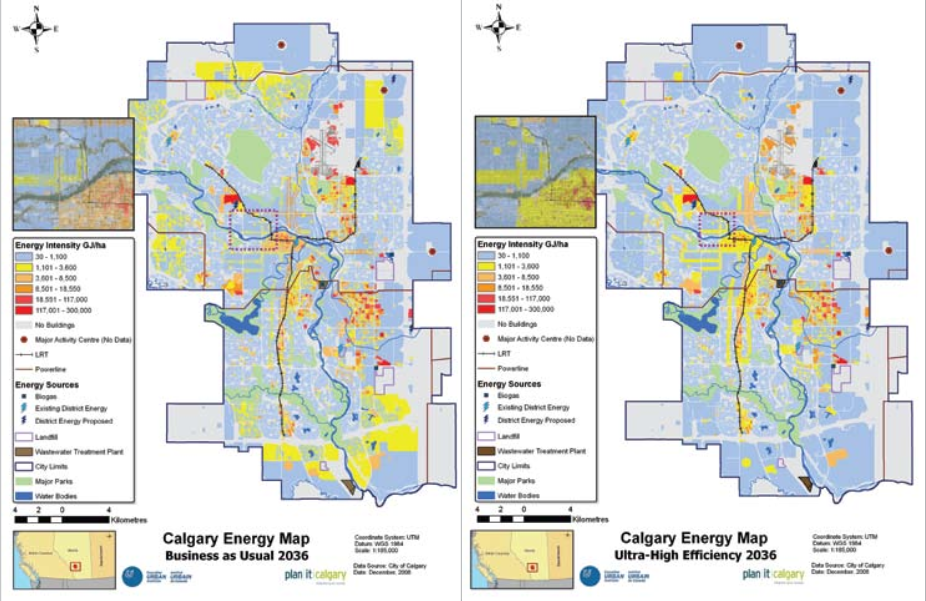
\includegraphics[width=0.6\linewidth]{calgaryCmp.png}
  \caption{Calgary Energy Map (Business as Usual, Ultra-High
    Efficiency)~\cite{aacip2009}}
  \label{fig:calgaryCmp}
\end{figure}

It also shows alternative energy sources of district energy, solar hot
water, solar air, energy sharing and PV installation on the map
(\fref{fig:calgaryAlter}). By overlaying the alternative technology
map and the ``ultra-high efficiency'' map, it highlights the
opportunities of using alternative renewable energy sources and
district energy system to further improve the energy performance of
high energy demand areas after high performance building design was
applied~\cite{aacip2009}.

\begin{figure}[h!]
  \centering
  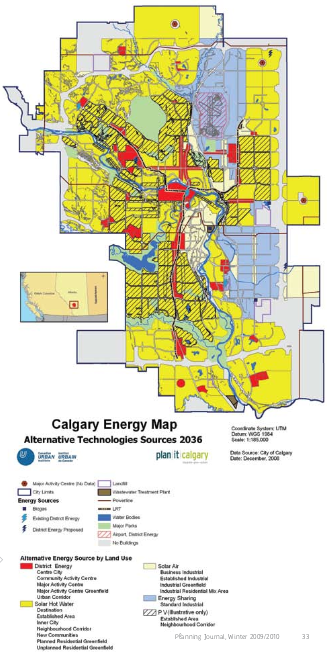
\includegraphics[width=0.3\linewidth]{calgaryAlter.png}
  \caption{Calgary Energy Map Alternative Energy Source~\cite{aacip2009}}
  \label{fig:calgaryAlter}
\end{figure}

\subsubsection{UK Heat Map}
Under the goal of supplying 25\% of the total energy with
decentralized energy (DE) by the year 2025, the Decentralised Energy
Master Planning Program (DEMaP) was conducted between 2008 to 2010 to
``identify opportunities for district heating networks through heat
mapping and energy masterplanning''~\cite{londonHeatMap}. In this
study, the term DE only refers to ``combined heat and power systems
connected to district heating
networks''~\cite{decentralHeatMap2011}. 

London Heat Map is a publicly accessible interactive map developed as
part of the DEMaP project. It is completed for the London Boroughs in
2012. It can act as a starting point of Energy Master Plan for local
authorities, and can assist developers to make connections to existing
DE networks to meet policy requirements (London Plan DE
policy)~\cite{decentralHeatMap2011, londonHeatMap}. Point features of
high heating energy consumers and suppliers, existing and emerging
energy networks are depicted on the interactive map. High DE potential
regions (``focus area''~\cite{decentralHeatMap2011}) are identified
and depicted on the map to highlight the opportunities of utilizing
the heat supply in the community planning and development
(\fref{fig:londonHeat}). The ``live-database'' property of London Heat
Map allows new data of energy consumption be uploaded by users.

The criteria applied for identifying focus area include: 1) near to
existing or emerging DE network, 2) high heat demand density 3) anchor
load building, 4) diverse heating demand profile 5) has public
ownership with policy concerns to make connections to the DE
network~\cite{decentralHeatMap2011}. The physical constraint are also
considered in finalizing the high DE potential regions.
\begin{figure}[h!]
  \centering
  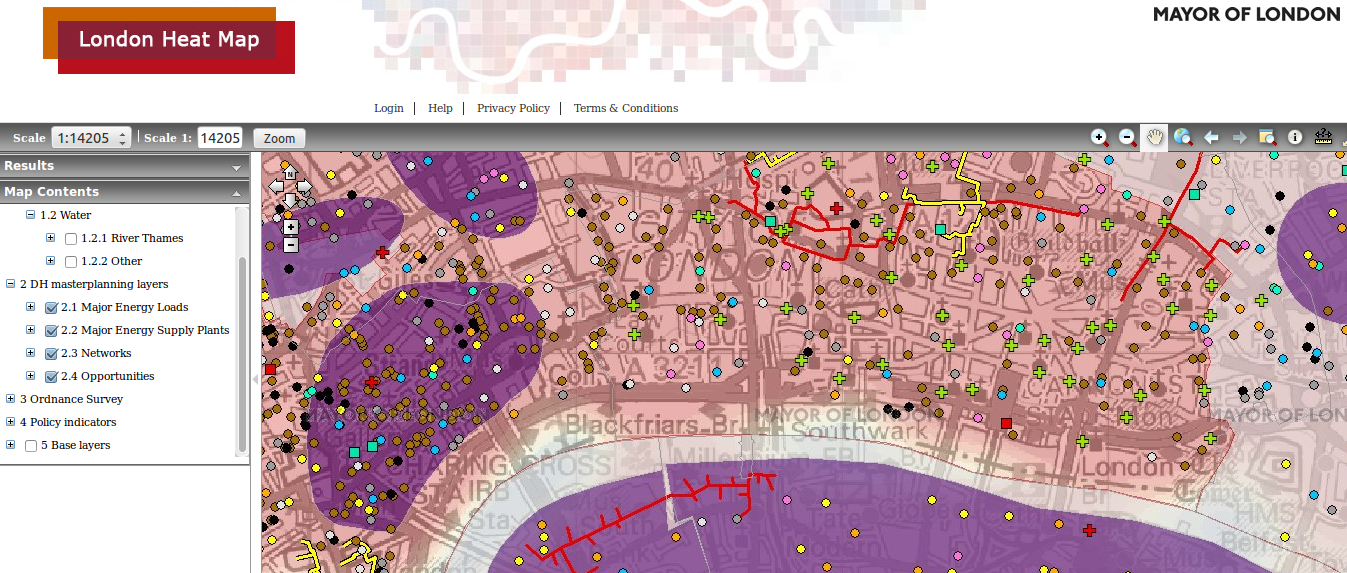
\includegraphics[width=0.7\linewidth]{londonHeat.png}
  \caption{London Heat Map~\cite{londonHeatMapMap}}
  \label{fig:londonHeat}
\end{figure}

National Heat Map (\fref{fig:nhm}) is another UK energy mapping
project that focuses more on the industry
side~\cite{decentralHeatMap2011}. It is a ``high resolution
web-based'' heating energy interactive map, developed by the
Department of Energy and Climate Change (DECC). It aims at ``support
planning and deployment of local low-carbon energy projects in
England''~\cite{heatMap2015}. Power plant developers can use this map
to consider the feasibility for a CHP plant under policy
requirements~\cite{decentralHeatMap2011}. Heating demand density
($kWh/m^2$) of four major building sectors: public buildings,
commercial buildings, industry buildings and residential buildings,
together with the total demand is plotted on the map as a 2D raster
image with a discrete color scheme from blue to red representing low
to high heating demand. Heat source of CHP stations and thermal power
stations are plotted as point features in the map. Address level heat
demand data in csv format is also available for local authorities upon
request~\cite{heatMapLocal2012}.

\begin{figure}[h!]
  \centering
  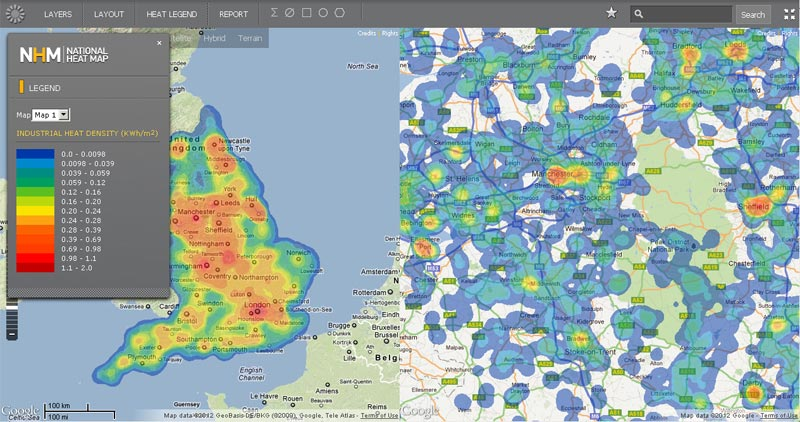
\includegraphics[width=0.5\linewidth]{nhm.jpeg}
  \caption{National Heat Map~\cite{heatMap2012}}
  \label{fig:nhm}
\end{figure}

The ``Water Source Heat Map'' (\fref{fig:waterMap}) is an added layer
group to the existing National Heat Map with information about the the
heat potential of the 4041 waterways in England. Heat potential of
waterways are represented in temperature, surface area, flow rate and
heat capacity ($kJ/m^3$ for coastal and estuary, $kW$ for canal, river
and settlement). It aims at supporting the plan of water-based thermal
system as water-based heat pump~\cite{waterHeatMap}. The map revealed
the large thermal capacity of water bodies that could serve over one
million buildings in the UK~\cite{waterHeatMap}.

\begin{figure}[h!]
  \centering
  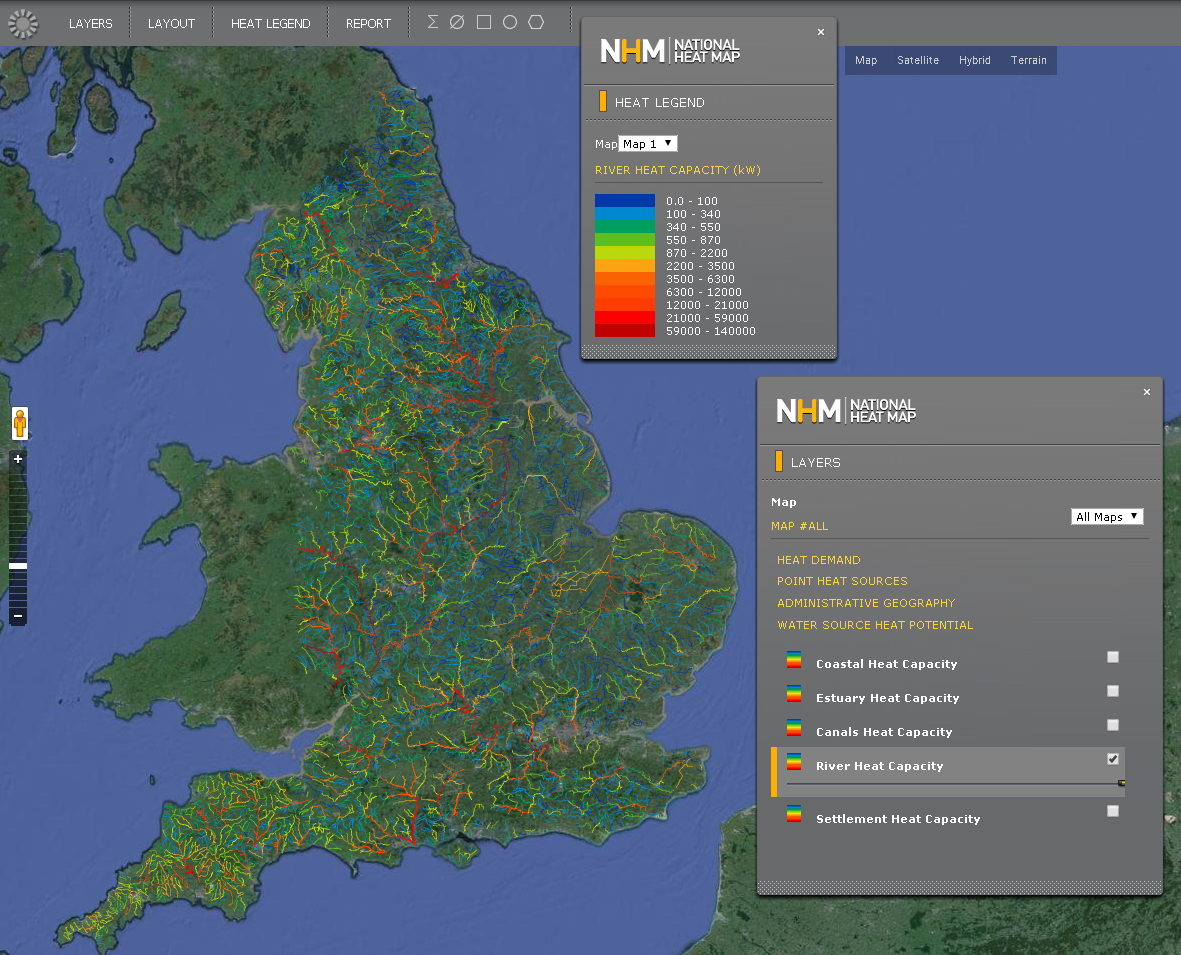
\includegraphics[width=0.5\linewidth]{waterMap.png}
  \caption{Water Heat Map~\cite{waterHeatMap}}
  \label{fig:waterMap}
\end{figure}

\subsubsection{Energy Potential Mapping}
Dobbelsteen et al. described a framework of Energy Potential Mapping
(EPM) that aggregates information of energy supply, demand and
infrastructure on the same map with demand and supply represented in
the same unit of GJ or GJ/ha~\cite{Dobbelsteen2013}.

In 2010, a ``Heat Mapping'' study under the framework of EPM was
launched by TU Delft aiming at visualizing heat demand and supply and
infrastructure with the same unit that facilitates easy comparison and
facilitates the matching of supply and
demand~\cite{Dobbelsteen2013}. The map is presented with aggregated
supply and demand in a 3D Heat Map. The absolute quantity of each type
of demand and supply is represented with extruded height in the 3D
map. Demand is represented with a transparent 3D feature, and each
supply source is represented with solid 3D feature in a different
color~\cite{Dobbelsteen2013}.

\begin{figure}[htbp]
  \centering
  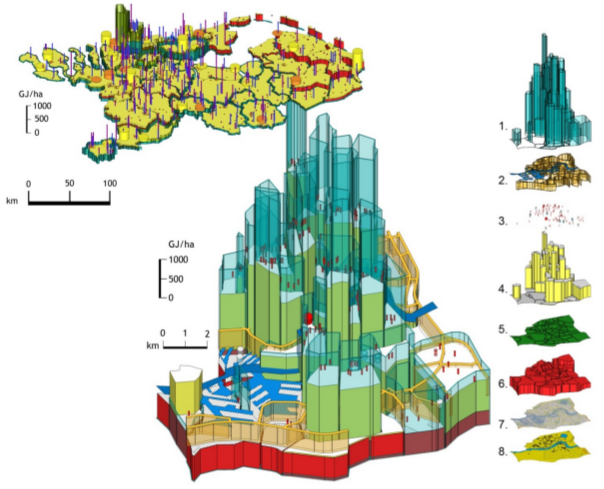
\includegraphics[width=0.7\linewidth]{heatmapNL.png}
  \caption{Heat Mapping of Netherlands and
    Rotterdam~\cite{Dobbelsteen2013}}
  \label{fig:heatmapNL}
\end{figure}

\subsection{Dynamic Energy Map}\label{dynamicMap}
As is discussed before, dynamic map includes time information in a
map. Several existing approaches occur.

\subsubsection{Lower Hill District Dynamic Mapping Project}
In 2011 to 2012, the Dynamic Energy Map of the Lower Hill District,
Pittsburgh, PA was created. It is designed to conduct feasibility
analysis and comparison of alternative energy supply techniques of a
district energy system~\cite{baird2014, Ramesh2013}. A geo-data base
was created with ArcMap, ArcScene and Sketchup. In the database, each
building, represented as a 3D feature, contains attributes of its
building name, annual energy consumption, energy use intensity (EUI),
and annual and monthly peak demand. The map is online accessible via
GIS Cloud (\fref{fig:mellonArenaGIS}).

\begin{figure}[h!]
  \centering
  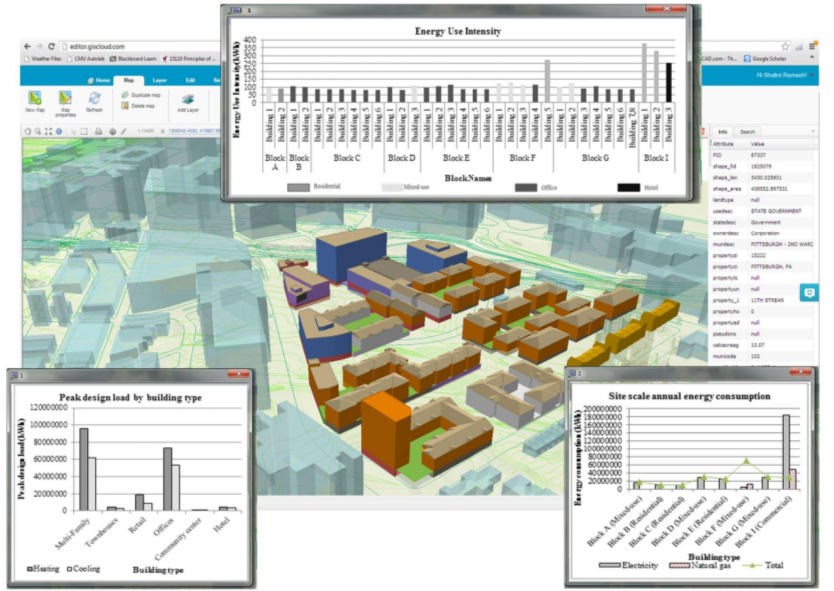
\includegraphics[width=0.7\linewidth]{mellonArenaGIS.png}
  \caption{Online Accessible GIS-database with GIS
    Cloud~\cite{baird2014, Ramesh2013}}
  \label{fig:mellonArenaGIS}
\end{figure}

The feasibility analysis and temporal data display are separated from
the geo-database and is performed in a excel screening tool. The tool
takes input of energy cost rate, building type and size, development
phase and central plant types and feature and produces a feasibility
analysis and related temporal graphs (\fref{fig:3dexcel}) of annual
hourly energy consumption for each building type and the aggregated
demand of natural gas, cooling use electricity and total electricity.

\begin{figure}[h!]
  \centering
  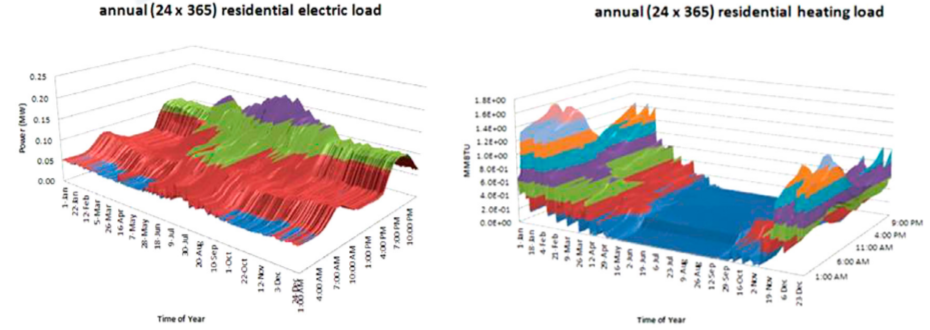
\includegraphics[width=0.7\linewidth]{3dexcel.png}
  \caption{Heating Load and Electricity Load for Residencial
    Building~\cite{baird2014}}
  \label{fig:3dexcel}
\end{figure}

\subsubsection{Energy Mapping to Identify Opportunities for Future
  Networks Project}
Another instance of energy demand dynamic map with high spatial
resolution was found in the project ``Energy Mapping to Identify
Opportunities for Future Networks''~\cite{Diaz2013}. The aim of the
project is to ``analyze the spatial and temporal distribution of
energy consumption'' and support decision making and design of energy
network: more specifically, to identifiy opportunities of District
Heating, CHP plant development and Building Design
Improvement~\cite{Diaz2013}.

Energy Demand Maps of three different resolutions were created using
QGIS: campus level, community level and city level. Energy data was
retrieved from both metered data (used in campus level map) and HEM
simulation (used in community and city level map). HEM is a tool for
``mapping the possiblemapping the possible carbon and energy
performance of a dwelling. It has pre-simulated results embedded as a
data table in the tool and applies the appropriate system and context
calculations to provide instant energy, carbon and cost results''~\cite{HEMesru2015}.

For the campus level map, the heat demand density (heat demand over
conditioned area) were depicted to identify ``outliers'': the
buildings with high heat demand~\cite{Diaz2013campus}. These outliers
were potential buildings need to be improved in building insulation
level or HVAC system efficiency. They claim a spatial map is
sufficient for this outlier identification process
(\fref{fig:heatGlasgow}). They also created a temporal spatial map of
monthly heat consumption that is in the form of both small multiples
(\fref{fig:seqheatGlasgow}) and non-interactive animated map
(\fref{fig:animeheatGlasgow}). With the dynamic map, they identified
two campus buildings with high heat demand through the whole year
(anchor load building) and concluded that the two buildings could
connect to a district heating system. They also created two animated
maps with electricity and natural gas. By comparing these two animated
maps, consistent high consumers for electricity and gas were
identified as potential candidate building for a micro-CHP
system~\cite{microCHP}.

\begin{figure}[h!]
  \centering
  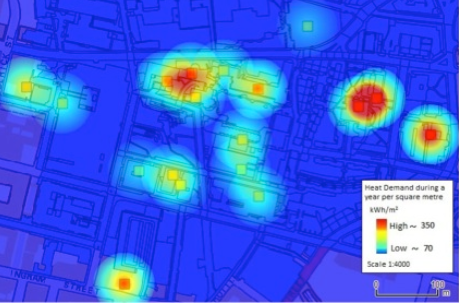
\includegraphics[width=0.5\linewidth]{heatGlasgow.png}
  \caption{Campus Level Heat Demand Density Map~\cite{Diaz2013campus}}
  \label{fig:heatGlasgow}
\end{figure}

\begin{figure}[h!]
  \centering
  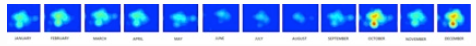
\includegraphics[width=0.5\linewidth]{seqheatGlasgow.png}
  \caption{Campus Level Monthly Heat Demand Map in Small Multiples\cite{Diaz2013campus}}
  \label{fig:seqheatGlasgow}
\end{figure}

\begin{figure}[h!]
  \centering
  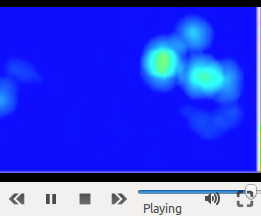
\includegraphics[width=0.3\linewidth]{animeheatGlasgow.png}
  \caption{Campus Level Monthly Heat Demand Map in Animation\cite{Diaz2013campus}}
  \label{fig:animeheatGlasgow}
\end{figure}

The community level spatial and temporal GIS analysis undertook a
similar process as the campus level except for the energy data is
retrieved from HEM simulation. By comparing the four different
building types: ``Traditional Build, New Build, Council Estate, High
Rise Flat'', they identified the consistent high gas and electricity
demand of High Rise Flat buildings. They also discovered that the
improvement of building design could adjust the heat to power ratio
(HTP) and could make applying CHP option feasible~\cite{Diaz2013com}.

City level map does not contain temporal mapping analysis and is left
out from the case study~\cite{Diaz2013city}.

\section{Building From Previous Work}
As is mentioned in the introduction, a dynamic energy map has four
major functions: 1) holding, 2) visualizing and 3) analyzing community
level high spatial-temporal resolution energy demand and supply data
4) connection to simulation engine for iterative performance
analysis. 

In the initial instance of Dynamic Energy Map by Baird et al.\
~\cite{baird2014}, function 1) of holding spatial-temporal (although
with low temporal resolution) energy data is realized by processing
the energy simulation data with Microsoft excel and importing the csv
file including ``building name, total conditioned area annual, energy
use intensity, annual and monthly peak demand''. The further
improvement of the current project is to make the geo-database hold
more high resolution energy data, meaning the 8760 hourly energy data
should be contained in the dynamic energy map.

Function 4) of connecting to building simulation data is also realized
by importing simulation result csv files to the geo-database (although
with low temporal resolution).

For function 3), the feasibility analysis of a district energy system
is performed in a stand-alone excel tool~\cite{baird2014} but it is
possible that the analysis result could be linked in to the
geo-database as the energy simulation result. 

For function 2), the spatial and temporal information are visualized
separately in the Lower District Hill Project: the spatial information
of 3D building geometry and location could be visually inspected in
the geo-database but not the hourly energy consumption information. 2)
The temporal visualization of energy demand is done separately in the
excel screening tool as 3D graphs, but no spatial context is present
and the spatial dimension is then lost. The authors thus identified
the crucially missing function: the visualization of such a
spatial-temporal changing of energy behavior as the major goal of the
current project.

\begin{figure}[h!]
  \centering
  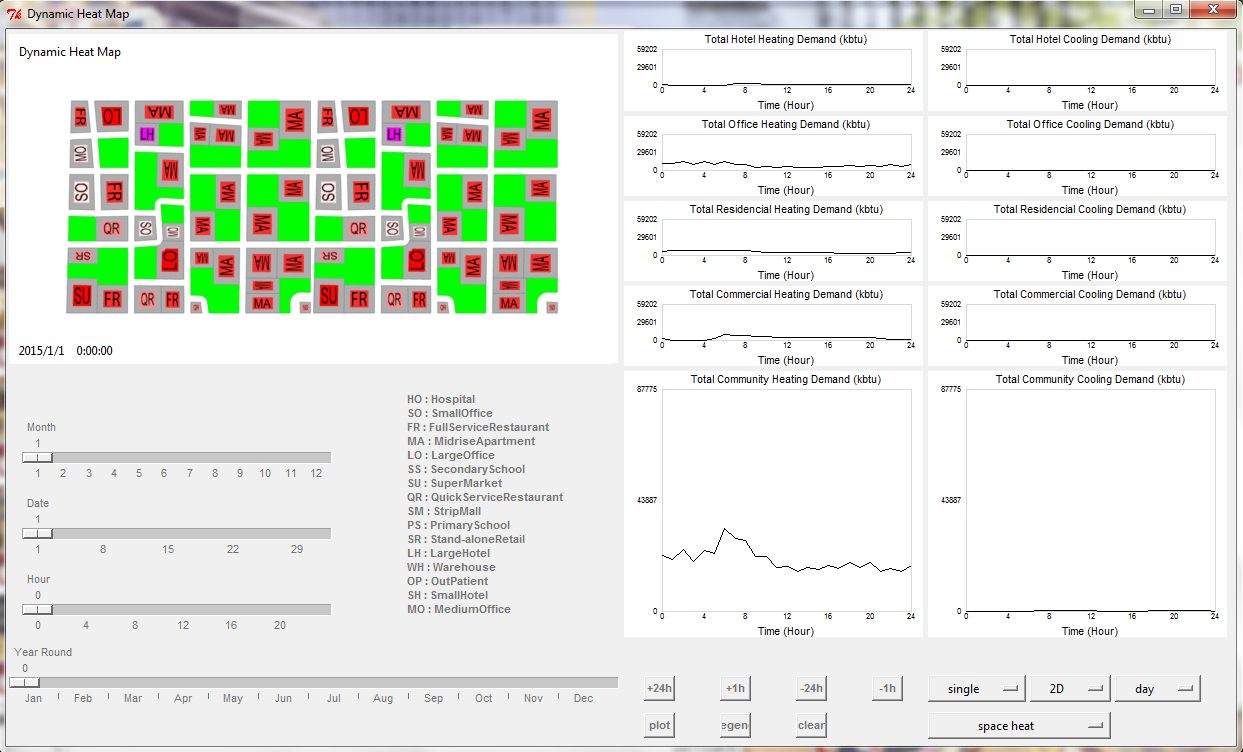
\includegraphics[width=0.7\linewidth]{interface08.png}
  \caption{Unified Dynamic Energy Map Display System}
  \label{fig:interface08}
\end{figure}

\pagebreak
\section{Methodology}\label{method}
\subsection{Overview}
The Dynamic Energy Map is created with a conceptual urban environment
whose building density and land use pattern resembles a redevelopment
project at Lower Hill District, Pittsburgh, PA~\cite{Ramesh2013}. The
number of buildings in the model represents a typical sized community
that can be served by a district energy system~\cite{IDEA2012}.

The inputs to the dynamic energy map are the energy consumption data
and the urban environment layout. For the conceptual setting, the
energy data is retrieved from the simulation of DOE Benchmark
buildings of new construction which comply with ASHRAE 90.1-2004
Standard~\cite{DOE2015}.

The urban environment layout is created so that it follows a typical
urban environment land use pattern. The output of the dynamic energy
map is a sequence of 2D or 3D energy choropleth maps images. 

An interface is designed to provide an interactive inspection of the
map sequence and create dynamic data plots (~\fref{fig:flow}). By
replacing the simulated energy data with actual metered energy
consumption data and the conceptual layout with a real urban
environment layout, the same method can be directly applied to the
analysis of a real project.

The major functions of the current program include: 
\begin{enumerate}[i.]
\item  comparing heating and cooling demand to identify energy recovery opportunities 
\item comparing heating and electricity demand to size co-generation system
\end{enumerate}

\begin{figure}[htbp]
  \centering
  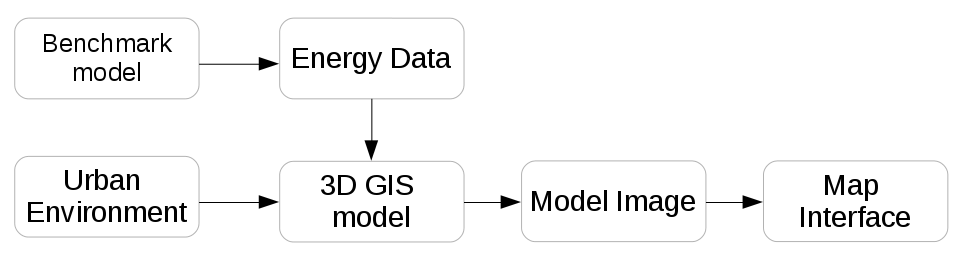
\includegraphics[width=0.7\linewidth]{flow.png}
  \caption{General Work Flow}
  \label{fig:flow}
\end{figure}

\newpage
\subsection{Input}
\subsubsection{Benchmark Models and Energy Data}
In the Lower Hill District project preliminary district system
feasibility analysis session, DOE benchmark buildings were substituted
for buildings in the community model. This approach allows for a fast
initial system assessment~\cite{baird2014}.

Following the same approach, the energy profile used in the current
study is retrieved from simulation results of commercial building
benchmark buildings developed by U.S. Department of Energy
(DOE)~\cite{DOE2015}. There are 16 building types in the benchmark
models (\fref{tab:doeModel}). The building types involved in the
current project include: Large Office (LO), Medium Office (MO), Small
Office (SO), Stand-alone Retail (SR), Supermarket (SU), Quick Service
Restaurant (QR), Full Service Restaurant (FR), Large Hotel (LH) and
Midrise Apartment (MA). The two-letter shorthand in the parenthesis
after each building type is used in the building label for the dynamic
map display. The general information for the benchmark buildings are
shown in \tref{tab:doeModel}:

\begin{table}[h!]
  \centering
  \begin{tabular}{l|l|c|c}
    \hline
Building Type Name&Shorthand&  Floor Area (ft2)    & Number of Floors\\
    \hline
Large Office	         &LO&  498,588	      & 12\\
Medium Office	         &MO&  53,628	      & 3\\
Small Office	         &SO&  5,500	      & 1\\
Warehouse	         &WH&  52,045	      & 1\\
Stand-alone Retail       &SR&  24,962	      & 1\\
Strip Mall	         &SM&  22,500	      & 1\\
Primary School	         &PS&  73,960	      & 1\\
Secondary School         &SS&  210,887	      & 2\\
Supermarket	         &SU&  45,000	      & 1\\
Quick Service Restaurant &QR&  2,500          & 1\\
Full Service Restaurant  &FR&  5,500          & 1\\
Hospital	         &HO&  241,351	      & 5\\
Outpatient Health Care   &OP&  40,946	      & 3\\
Small Hotel	         &SH&  43,200	      & 4\\
Large Hotel	         &LH&  122,120	      & 6\\
Midrise Apartment        &MA&  33,740	      & 4\\
    \hline
\end{tabular}
\caption{DOE Benchmark Building General Information~\cite{DOE2015}}
\label{tab:doeModel}
\end{table}

The benchmark buildings comply with the ASHRAE Standard 90.1-2004. The
HVAC system types are shown in \tref{tab:hvac}. The major heating
systems of the benchmark buildings are furnace and boilers, except
that the small hotel and the warehouse has individual space heaters
other than furnace. The cooling systems are chillers for Large Hotel
(air-based) and Large Office (water-based) and PACU (packed
air-conditioning unit) for other building types.~

\begin{table}[h!]
\centering
\scriptsize
\caption{Benchmark Building HVAC System}
\label{tab:hvac}
%\begin{tabular}{l|p{3cm}|p{4cm}|p{4cm}}
\begin{longtable}{l|p{3cm}|p{4cm}|p{4cm}}
  \hline
  & Heating                                & Cooling                                                                     & Air                                                     \\
  \hline
  \hline
  Small Office             & Furnace                                & PACU (packed air-conditioning unit)                                         & SZ CAV (single-zone constant air volume)                \\
  \hline
  Medium Office            & Furnace                                & PACU (packed air-conditioning unit)                                         & MZ VAV (multizone variable air volume)                  \\
  \hline
  Large Office             & Boiler                                 & Chiller (2) water cooled                                                    & MZ VAV (multizone variable air volume)                  \\
  \hline
  Primary School           & Boiler                                 & PACU (packed air-conditioning unit)                                         & CAV (constant air volume)                               \\
  \hline
  Secondary School         & Boiler                                 & Chiller (2) air cooled                                                      & MZ VAV (multizone variable air volume)                  \\
  \hline
  Stand-Alone Retail       & Furnace                                & PACU (packed air-conditioning unit)                                         & SZ CAV (single-zone constant air volume)                \\
  \hline
  Strip Mall               & Furnace                                & PACU (packed air-conditioning unit)                                         & SZ CAV (single-zone constant air volume)                \\
  \hline
  Suprmarket               & Furnace                                & PACU (packed air-conditioning unit)                                         & SZ CAV (single-zone constant air volume)                \\
  \hline
  Quick Service Restaurant & Furnace                                & PACU (packed air-conditioning unit)                                         & CAV (constant air volume)                               \\
  \hline
  Full Service Restaurant  & Furnace                                & PACU (packed air-conditioning unit)                                         & SZ CAV (single-zone constant air volume)                \\
  \hline
  Small Hotel              & ISH (individual space heater), furnace & IRAC (individual room air conditioner), PACU (packed air-conditioning unit) & SZ CAV (single-zone constant air volume)                \\
  \hline
  Large Hotel              & Boiler                                 & Chiller (2) air cooled                                                      & FCU (Fan Coil Unit) and VAV (variable air volume)       \\
  \hline
  Hospital                 & Boiler                                 & Chiller (2) water cooled                                                    & CAV (constant air volume) and VAV (variable air volume) \\
  \hline
  OutPatient Healthcare    & Furnace                                & PACU (packed air-conditioning unit)                                         & CAV (constant air volume) and VAV (variable air volume) \\
  \hline
  Warehouse                & ISH (individual space heater), furnace & PACU (packed air-conditioning unit)                                         & SZ CAV (single-zone constant air volume)                \\
  \hline
  Midrise Apartment        & Furnace                                & PACU-SS                                                                     & SZ CAV (single-zone constant air volume)               \\
  \hline
\end{longtable}
\end{table}

\pagebreak
\paragraph{Input for Identifing Energy Recovery Opportunities}
The major heat rejection sources include heating mode heat rejection
and cooling mode heat rejection. The heat rejection in heating mode
happens during the process of the mixing of conditioned and outside
air. The heat rejection in cooling mode happens at the condensing
process when the high temperature refrigerant gas condenses with one
of the following heat rejection forms~\cite{Bhatia2015}:
\begin{itemize}
\item Air cooled unit: ambient air is blown through condensing coils
  and removes heat from the gas refrigerant.
\item Cooling tower: cooled water flow past the condensing unit and
  takes away the heat from the gas refrigerant. The water is then
  cooled through evaporation.
\item Fluid cooler: water is sprayed on the condensing coil with fan
  forced air flowing in the opposite direction as the water. It
  causes evaporation cooling effect that takes away the heat from the
  gas refrigerant. 
\end{itemize}
The heat ``condenser total heat of rejection''~\cite{Bhatia2015} (THR)
in the condensing process equals to the ``net refrigeration effect''
~\cite{Bhatia2015}(RE), which is the hourly cooling demand, plus the
compressor input, it can be represented as the following equation:

$$THR = RE * f$$

$f$ is the ``Heat Rejection Factor'' and it is typically between 1.15
and 1.25~\cite{Bhatia2015}. The water-based system has heat rejection
factor closer to 1.15 and air-based system closer to
1.25~\cite{Bhatia2015}.

To help users identify energy recovery opportunities, the energy
information needed to retrieve include: space heating energy demand
and space cooling energy demand, which is an indicator for heat
rejection that could be recovered and shared within a single building
or a building group.

From \tref{tab:heatFuel}, Large Hotel, Medium Office, Midrise
Apartment, OutPatient Healthcare, Small Hotel and Stand-alone Retail
use both electricity and natural gas for space heating, the rest of
the building types uses only natural gas for space heating. We thus
use the EnergyPlus simulation output parameters
``heating:electricity'' and ``heating:gas'' to represent the space
heating demand of reference buildings.
\begin{table}[h]
\centering
\caption{Annual Total Heating Demand by Fuel Type}
\label{tab:heatFuel}
\begin{tabular}{lll}
  \hline
                       & Electricity {[}kBtu{]} & Gas {[}kBtu{]} \\
  \hline
  \hline
FullServiceRestaurant  & 0.0                    & 856637.1       \\
Hospital               & 0.0                    & 14045664.0     \\
LargeHotel             & 843.6                  & 2960506.8      \\
LargeOffice            & 0.0                    & 4741180.3      \\
MediumOffice           & 450791.3               & 192226.8       \\
MidriseApartment       & 56.9                   & 494959.6       \\
OutPatient             & 199581.9               & 2881638.9      \\
PrimarySchool          & 0.0                    & 1579186.5      \\
QuickServiceRestaurant & 0.0                    & 383297.2       \\
SecondarySchool        & 0.0                    & 7746443.0      \\
SmallHotel             & 52129.9                & 450393.2       \\
SmallOffice            & 0.0                    & 66631.5        \\
Stand-aloneRetail      & 6966.5                 & 976583.4       \\
StripMall              & 0.0                    & 1013188.1      \\
SuperMarket            & 0.0                    & 3043905.2      \\
Warehouse              & 0.0                    & 1039850.2     \\
  \hline
\end{tabular}
\end{table}

\begin{figure}[h!]
  \centering
  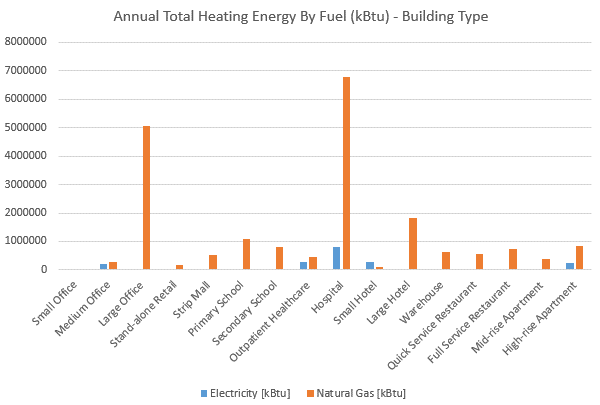
\includegraphics[width=0.7\linewidth]{heatFuel.png}
  \caption{Heating Fuel}
  \label{fig:heatFuel}
\end{figure}
Electricity is the only fuel used for space cooling, thus the
EnergyPlus output parameter ``cooling:electricity'' is used to
represent space cooling demand. According to the suggested heat
rejection factor~\cite{Bhatia2015}, the heat recovery potential will
be calculated with $f = 1.15$ for Large Office and Hospital, and
$f = 1.25$ for the remaining building types:
$$\text{Heat Recovery Potential} = \text{cooling:electricity} \times f$$

In summary, to facilitate identification of energy recovery
opportunities for single buildings and within building groups, the
hourly ``heating:electricity'', ``heating:gas'' and
``cooling:electricity'' output will be extracted from energyPlus
simulation of DOE Commercial benchmark buildings.

\paragraph{Input for Sizing District Co-generation System}
For the sizing of a district co-generation system, the relevant
information needed are the total heating demand, and the total
electricity demand. The general principle used in Lower Hill District
project ~\cite{baird2014} is to use the minimum total heat demand
(space heating and service hot water) over time to assess the minimum
capacity of electricity generation ($E_{heat}$) such that its heat
bi-product from electricity generation will always be consumed. The
maximum total electricity demand ($E_{elec}$) is used for assessing
the capacity of a backup system or a second phase system development
by $C_{backup} = E_{elec} - E_{heat}$ where $C_{backup}$ is the
capacity of electricity generation for the backup system or
second-phase development.

Heating demand assessed in the sizing of co-generation system is
different from the energy recovery use case. It contains the space
heating demand and the service hot water demand. From the summary
files of benchmark models, the fuel used for providing service hot
water is natural gas for all building types (\tref{tab:hotWater})
\begin{table}[h!]
\centering
\caption{Service Hot Water by Fuel Type}
\label{tab:hotWater}
\begin{tabular}{l|l|l}
  \hline
                       &  Electricity {[}kBtu{]} & Gas {[}kBtu{]} \\
  \hline
  \hline
FullServiceRestaurant  & 0 & 253664.3       \\
Hospital               & 0 & 719402.7       \\
LargeHotel             & 0 & 6793934.2      \\
LargeOffice            & 0 & 231381.1       \\
MediumOffice           & 0 & 34178.3        \\
MidriseApartment       & 0 & 289719.3       \\
OutPatient             & 0 & 44054.5        \\
PrimarySchool          & 0 & 174768.0       \\
QuickServiceRestaurant & 0 & 82071.5        \\
SecondarySchool        & 0 & 441512.2       \\
SmallHotel             & 0 & 394017.1       \\
SmallOffice            & 0 & 10928.3        \\
Stand-aloneRetail      & 0 & 0.0            \\
StripMall              & 0 & 0.0            \\
SuperMarket            & 0 & 23799.7        \\
Warehouse              & 0 & 0.0            \\
  \hline
\end{tabular}
\end{table}

The output parameter ``electricity:facility'' was extracted to
represent the total electricity demand.

\pagebreak
\subsubsection{3D GIS Model Geometry}
The conceptual community model is constructed in
CityEngine~\cite{cityEngine2015}. CityEngine is a software developed
by Esri. It can aggregate geographic information into buildings and is
capable of smoothly transition models to ArcGIS\cite{ArcGIS2015}, one
of the widely applied tools for Geo-referenced data presentation and
analysis. Buildings in CityEngine is defined with ``rules'' using CGA
(Computer Generated Architecture) shape grammar that is unique to
CityEngine. The rule-based modeling of urban environment enables fast
construction and easy adjustability of urban density, skyline and
terrain control. It also enables easy aggregation of Energy profile
data into 3D urban environment models.

Although the urban environment in this study is a conceptual setting,
we still want it to reflect the topological and density pattern in a
real urban environment. To construct the model, we first extracted the
topological pattern from an existing urban design project, the Mellon
Arena Project~\cite{baird2014} (\fref{fig:mellonArena}.  There are
eight building types in the project: Residential (43\%), Town House
(2.9\%), Community Center (0.4\%), Commercial (3.8\%), Office (19\%),
Hotel (4.7\%), Cinema (1.4\%) and Garage (24.7\%).
\begin{figure}[h!]
  \centering
  \begin{subfigure}
  \centering
  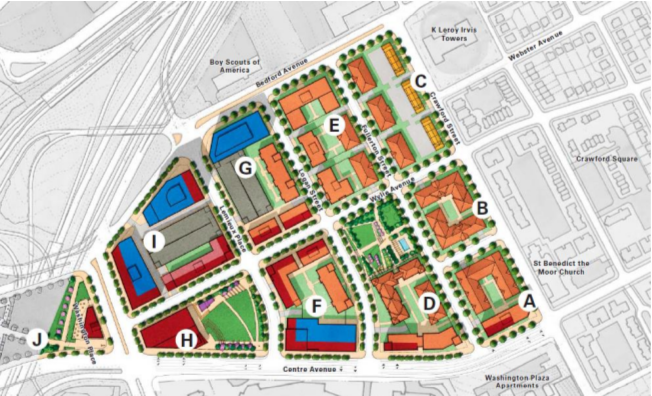
\includegraphics[width=0.5\linewidth]{mellonArena}
  \caption{Mellon Arena Project Site Plan View}
  \label{fig:mellonArena}
\end{subfigure}
~
\begin{subfigure}
  \centering
  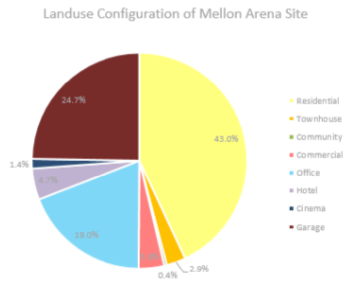
\includegraphics[width=0.3\linewidth]{mellonPie}
  \caption{Mellon Arena Site Land use Configuration}
  \label{fig:mellonPie}
\end{subfigure}
\end{figure}
The 16 building types in DOE commercial benchmark models do not
perfectly correspond to those in the Mellon Arena Site. In order to
adapt the topological pattern of the Mellon Arena Project, a mapping
(function) from building types of Mellon Arena Site to building types
of DOE models is created as is shown in \tref{tab:typeMap}.
\begin{table}[h!]
  \centering
  \begin{tabular}{c| c| c}
    \hline
    Mellon Arena Type &Probability &DOE Building Type\\
    \hline
    Hotel &50\%&Large Hotel\\
    \cline{2-3}
    &50\%&Small Hotel\\
    \hline
    Office &30\%&Large Office\\
    \cline{2-3}
    &30\%&Medium Office\\
    \cline{2-3}
    &30\%&Small Office\\
    \hline
    Residential &100\%&Midrise Appartment\\
    \cline{1-2}
    Townhouse &100\%&\\
    \hline
    Commercial &25\%&Full Service Restaurant\\
    \cline{2-3}
    $+$ Cinema $+$&25\%&Quick Service Restaurant\\
    \cline{2-3}
    Community &25\%&Super Market\\
    \cline{2-3}
    Center &25\%&Stand-alone Retail\\
    \hline
  \end{tabular}
  \caption{Mapping of Mellon Arena to Building Types of DOE benchmark model}
  \label{tab:typeMap}
\end{table}

The four major building sectors involved in the current project are
residential, commercial, office and hotel. Their topological pattern
is represented in Figure \ref{fig:mellonTop}. The conceptual model
construction follows the building type topological pattern and the
urban density as the Mellon Arena Project (\fref{fig:sitePlan})
\begin{figure}[h!]
  \centering
  \begin{subfigure}
  \centering
  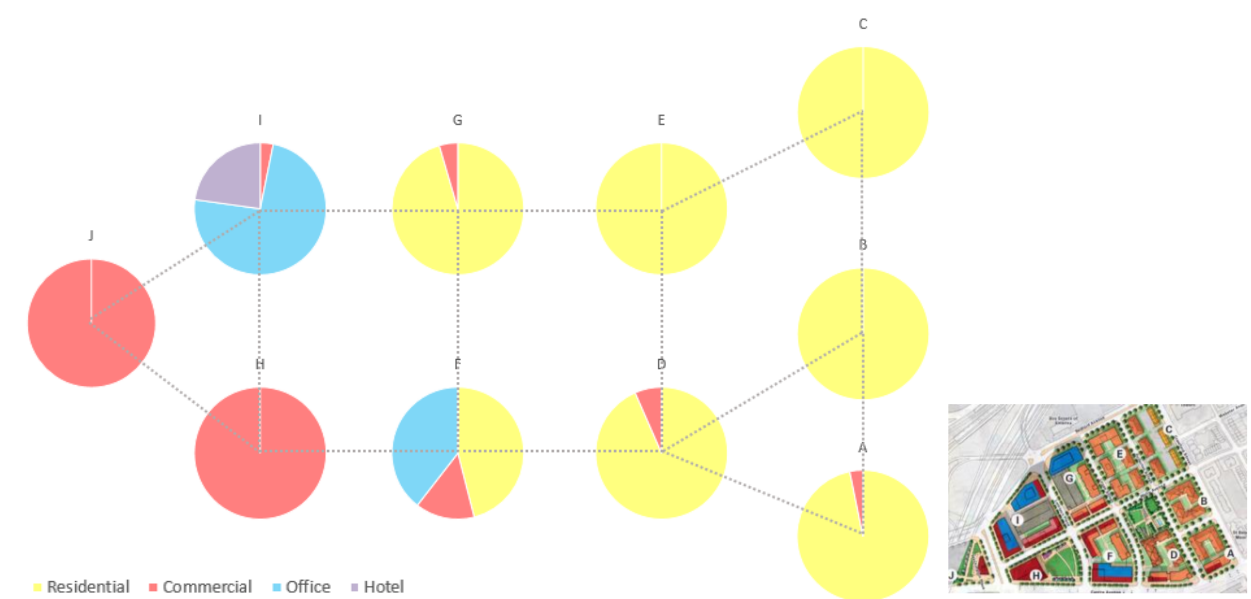
\includegraphics[width=0.7\linewidth]{mellonTop}
  \caption{Building Type Topological Pattern, Mellon Arena}
  \label{fig:mellonTop}
  \end{subfigure}
  ~
  \begin{subfigure}
  \centering
  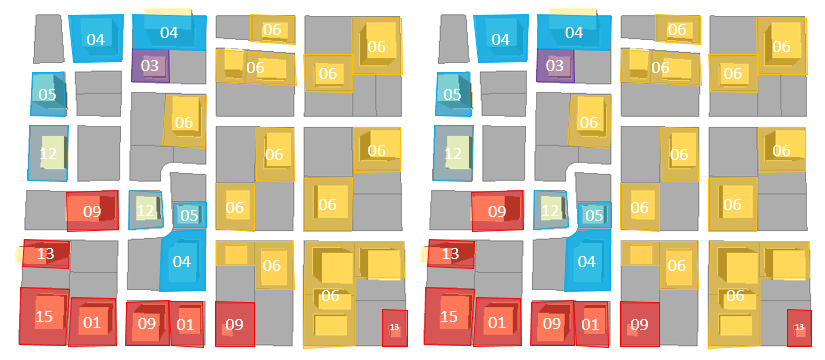
\includegraphics[width=0.7\linewidth]{sitePlan}
  \caption{Site Plan of Conceptual Model}~ (01: Full Service
  Restaurant, 03: Large Hotel, 04: Large Office, 05: Medium Office,
  \\06: Midrise Apartment, 09: Quick Service Restaurant, 12: Small
  Office, \\13: Stand-alone Retail, 15: Super Market)
  \label{fig:sitePlan}
  \end{subfigure}
\end{figure}   

\begin{comment}
\subsection{Data Collection and Analysis}
\subsubsection{Simulation Data Analysis of the benchmark
  models}\label{boxPlot}
The output of EnergyPlus simulation of 16 benchmark buildings are read
and processed with python script. This data loading and processing
module is used in both data analysis and the dynamic plot in the
interface design.

By analysing the EnergyPlus~\cite{EnergyPlus2015} simulation result of
the Heating Energy (Gas) and the Cooling Energy (Electricity), we
observed a large variation between different building types in these
two types of thermal energy demand.

Hourly heating demand of the benchmark building types involved in the
current model range from 0 to 12000 kBtu. The majority (75\%) of all
hourly consumption are below 2000 kBtu. All building types have a
large amount of outliers on the upper side. This indicates heating
demand of all building types are right skewed. The building type with
highest median heating demand are Large Hotel and Super Market. These
two building types could become the major ``heat sink'' or anchor load
building to be connected to a district system. In terms of peak
demand, Large Office has the highest peak heating demand
(\fref{fig:heatBox}).

Hourly cooling demand benchmark building types involved in the current
model range from 0 to 2500 kBtu, which is about 20\% of that of the
peak heating demand. Large Hotel has no outliers on the upper side,
meaning its hourly consumption are not as right skewed. Only Large
Hotel has non-zero median cooling demand (about 600 kBtu), meaning it
is the only building that has persistent cooling demand all year-round
. The design impact is: Large Hotel can act as an anchor building for
cooling if the central plant is a heating-cooling combined system that
can supply cooling energy as well. The consistent high cooling load of
Large Hotel also indicate a high portion of heat rejection. The reject
heat could be recovered and reused if building with moderate heating
demand are placed near the heavy cooling consumers
(\fref{fig:coolBox}).

The aggregated analysis above intends to provide a basic understanding
of the energy profile data distribution involved in the current
project. We anticipate to acquire more information than these
aggregated statistics with Dynamic Energy Map.

\begin{figure}[h!]
  \centering
  \begin{subfigure}
  \centering
  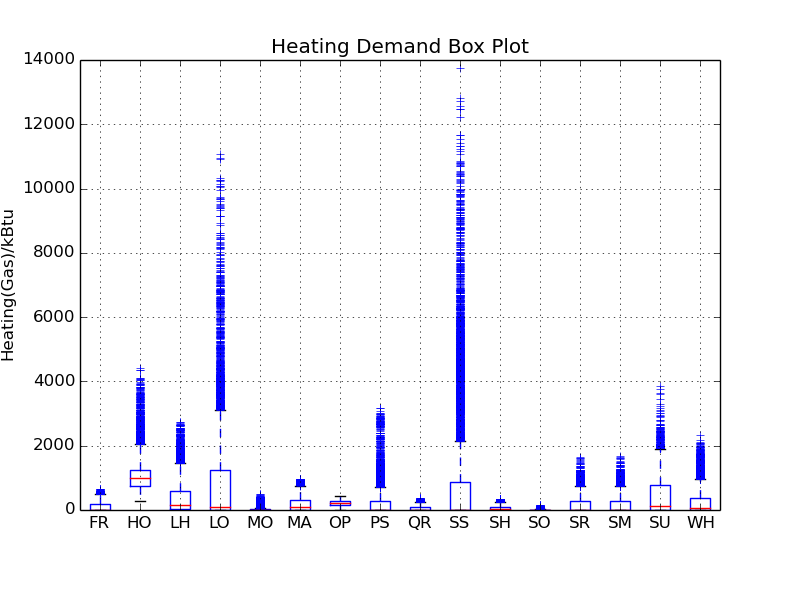
\includegraphics[width=0.7\linewidth]{heatBox}
  \caption{Heating Demand Box Plot}
  \label{fig:heatBox}
  \end{subfigure}%
  ~
  \begin{subfigure}
  \centering
  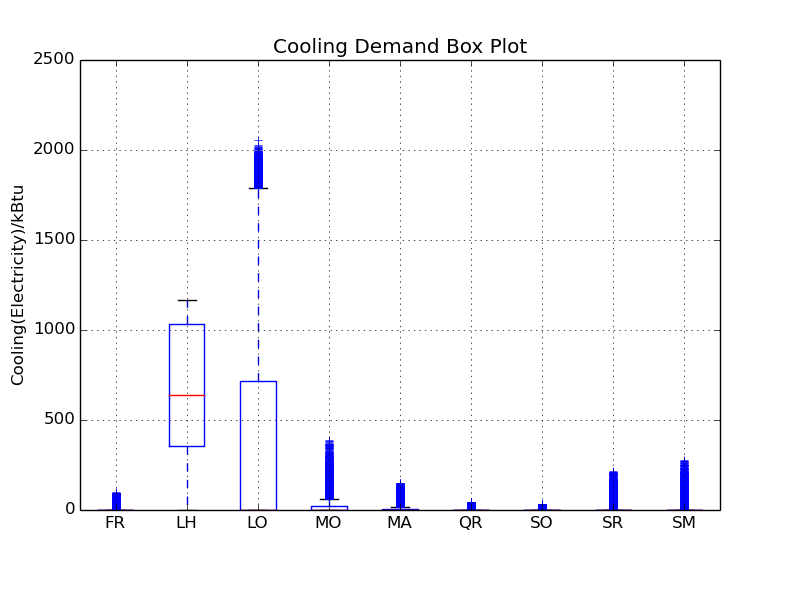
\includegraphics[width=0.7\linewidth]{coolBox}
  \caption{Cooling Demand Box Plot}
  \label{fig:coolBox}
  \end{subfigure}
\end{figure}   

\subsection{Temporal Data Aggregation}
The authors have experimented with two approaches to aggregate energy
profile data into the conceptual model constructed in CityEngine: 1)
write the energy profile data directly in the rule file for building
generation in CityEngine 2) importing 3D models from CityEngine to
ArcScene and aggregate the energy data into the 3D feature with
``one-to-many'' join.

The second approach has the advantage of 1) ready-to-use data
classification method and map symbol templates that facilitates
choropleth map design 2) the ``time-slider'' function for creating a
time-wise navigation and animated map. \fref{fig:arcgisTime} shows the
interface slider and the dynamic map of heating energy demand for the
conceptual model using ArcGIS. There are several problems of this
approach: 1) its high requirement of computational power makes it
infeasible to view on a normal PC. 2) The time dimension only exist
inside the map file. Although the animated map can be exported, the
output animation contains neither any form of temporal label nor the
control of playback. 3) For 3D GIS model, it does not contain a proper
function to extract single frames of map images, making it impossible
to implement exterior interface that deals with 3D maps.

The first approach, on the contrary, provides more flexibility but
also requires much user-end work including: pre-processing of energy
profile data, implementing data classification method and the
bivariate color ramp. An interface is also needed for visualising the
image sequence.

\begin{figure}[h!]
  \centering
  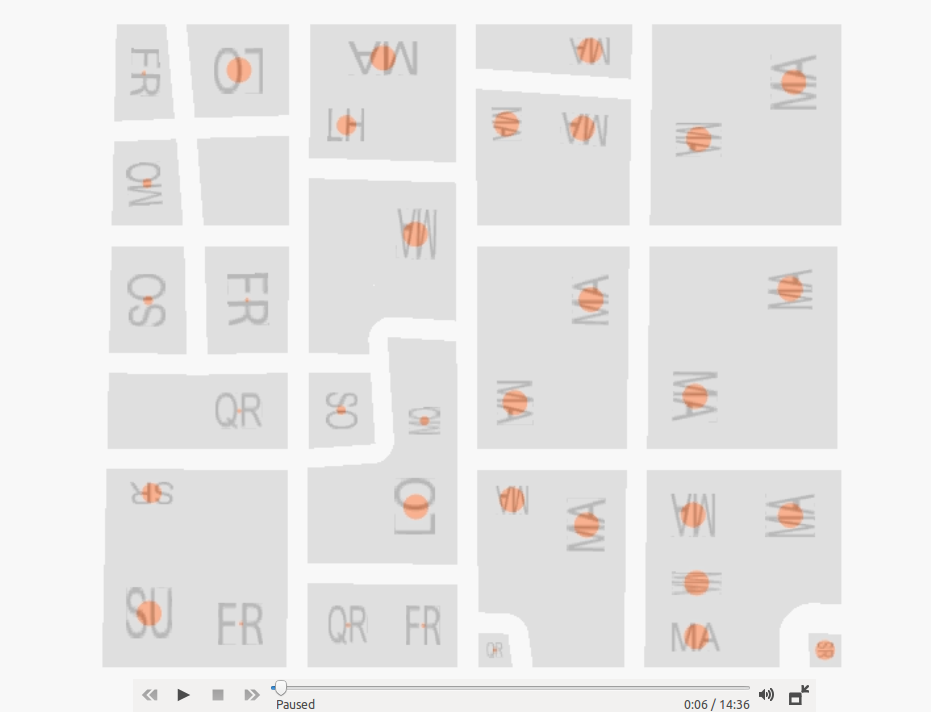
\includegraphics[width=0.5\linewidth]{arcgisTime}
  \caption{ArcGIS Time Slider for Temperal Data Display}
  \label{fig:arcgisTime}
\end{figure}

Due to limited time, the experimented GIS software are only restricted
to ArcGIS and CityEngine. There could be better alternatives to
achieve a dynamic map with more elegance. Find a better alternative
software to implement a dynamic map could be part of the work of the
next stage of the project.

\newpage
\subsection{Interface Specification}\label{interfaceSpec}
\subsubsection{User Definition}
We want to specify a user profile in order to best convey the
information with the Dynamic Energy Map.

The major category of user group for the Dynamic Map includes: 1)
policy makers, 2) urban planners with the interest in executing
community level energy strategys 3) researchers in energy related
fields 4) public groups or individuals that are involved or interested
in the decision making process of community energy planning.

The target user for the current interface design is restricted to
researchers in energy related fields. The assumption on this user
group about their skill level and background knowledge is that 1) they
have the basic ability to read and understand the layout of a map
environment and can associate it with the urban environment setting
they are associated with 2) they have the ability to correctly
understand moderately complicated map legend and data plot 3) they
have the basic understanding of related concept of building energy
performance attribute and the general implications of these
attributes. The assumptions about their intention is that they might
have different research interest and focus. These assumptions implies
the interface design should: 1) provide both qualitative and
quantitative information; 2) allow for some degree of user control
over data classification, legend selection and full control over time
navigation

\subsubsection{Goal Function}
The goal function of the interface is defined as: ``\textbf{Revealing
  the spatial-temporal heating and cooling demand variation of the
  conceptual model with Dynamic Energy Map}.''

As is mentioned in section \ref{districtDesign}, with the Dynamic
Energy Map that depict the spatial temporal load variation, one will
idealy be able to 1) idendify anchor load building, 2) conduct better
design of local load balancing, 3) identify energy recovery
opportunities of the following forms: an individual building with
mixed heating or adjacent buildings with opposite heating and cooling
demand.

\begin{enumerate}[1).]
\item Identify anchor load building
  
  To achieve this function, the map should be able to make the
  building with persistant high heating or cooling demand stand
  out. Thus the design of color scheme that assigns vibrant colors to
  high demand and white to low demand. The break points of ``high''
  demand remains to be decided in further project development. For the
  current implementation, the break point is acquired with quantile
  classification method with.

\item Local load balancing
  
  To achieve this, the first step would be to enable users to select a
  subset of the existing buildings and the program will calculate the
  aggregated maximum load and the load variation of the selected
  building group within the specified time period.

  The next step is to provide a utility that finds the optimal
  partition of the buildings in the urban environment that has the
  minimum load variance ratio within the group difference. A brute
  force approach would be:

  \begin{enumerate}[{Step }I.]
  \item Generate an adjacency table (dictionary) from the collection of
    building lot polygons with the key being building lot centroid labels.
  \item Create all legal partitions of the set of building centroids
    based on the adjacency table (i.e. a partition that includes a
    multi-part feature is not a legal partition)
  \item Calculate the sum of the load variation ratio for each of the
    legal partition. The load variation ratio for each subset of the
    element in a partition (a group of building) equals
    $${\text{max aggregated load} - \text{min aggregated load} \over \text{max aggregated
      load}}$$
  \item Find the partition with the minimum sum of load variation ratio
  \end{enumerate}
  
\item Identify energy recovery opportunities

  To achieve this, the heating and cooling demand should be
  represented on the same map that better depict the correlation.

\end{enumerate}

\subsubsection{Specification of the Major Operation}
The desired major operations for the target user include: 
\begin{itemize}
\item Map display and data plot
\item Navigation utilities that navigates through dynamic map and data
  plot
\item Provide default settings for choropleth map display
\end{itemize}

\paragraph{Map display and data plot}
For researchers or planners: The desired map display should be a 2D
and 3D map (providing easy toggle between 2D and 3D map or align the
two representations side by side) with graduated symbol or color
representing the heating or cooling demand. The map display should
also be coupled with corresponding data plot or data statistics that
providing the quantitative insight that supports design decisions.

For general public: The desired map display should be a 3D map
. Instead of using data plot, a more intuitive bar chart of the
aggregated demand could be more helpful in presenting a general
idea. The bivariate choropleth map legend should also be replaced with
two color ramps or even with only colors of extreme value. The data
classification method should also be chosen so that the peak
occurrence time is emphasized rather than the absolute energy
consumption value.

\paragraph{Navigation utilities that navigates through dynamic map
  and data plot}
The ability to navigate through a series of map images and present
dynamic data plot accordingly, is the basic function that differs
the current work from a static map. Some desired behavior of the
slider includes:
\begin{itemize}
\item Linear and cyclic time representation. According to section
  \ref{anime}, the time has both linear and cyclic aspect. The time
  navigation utility should provide both ``linear'' time navigation
  and ``cyclic'' time navigation. This requires a global time
  navigation that accounts for the linear aspect: it can go through
  the whole time period with the highest time resolution. It also
  requires a series of default time steps settings corresponding to
  the natural recurring pattern of the energy usage profile
\item Another desired feature is providing adjustable auto-play of the
  map animation. The reasoning behind this is the debatable level of
  user control in the study of Johnson and Nelson~\cite{Nelson1998},
  when they argue that allowing arbitrary time control might degrade
  the ability of animated map on conveying temporal pattern. This
  feature is to be implemented in future development of the project.
\end{itemize}

\subsubsection{Provide default settings for choropleth map display}
Creating several default settings for choropleth map display,
i.e. provide choices for data classification and color mapping. For
the current implementation, the variables in display is the heating
and cooling energy consumption profile. The customization choices only
restrict to the two classification method: even or quantile
method. The color ramp is predefined to be a bivariate color ramp from
white to red and blue. For later stages, a desired behavior would be
to provide the full control of color settings.

\subsubsection{Guidelines from Literature Study}
Here we summarizes some of the design choices made according to
related literature research on dynamic map design:
\begin{itemize}
\item Provide both 2D and 3D map display as a result of the debating
  situation mentioned in section \ref{2d3d}.
\item Choose bivariate choropleth map representation which has the
  highest accuracy rate in map reading experiments~\cite{Elmer2012}.
\item Providing the most commonly used data classification method:
  Equal Interval and Quantile Interval~\ref{dataClassification}
\item The number of classes for energy data classification is chosen
  to be 7, less than the suggested value of 10 as a result of smaller
  display size than 1024x768~\cite{doi:10.1559/1523040639298}
\item Provide both linear and periodical navigation based on section
  \ref{timeRepresent}
\item Using the principle of ``dual coding''~\cite{Resch2014} to
  assist legend reading by section \ref{anime}.
\item Noise removal in map display of energy profile
  data~\cite{Dorling1992}. This is done through the discrete color
  scheme design.
\end{itemize}

\subsection{Interface Design}\label{interfaceDesign}
\subsubsection {General Layout}
The interface for dynamic map display includes three major sections: a
series of sliders for controling images are on the left and the data
plot of energy profile of building sectors and aggregated demand are
on the right.

The main window on the top left is used for displaying the 2D dynamic
map of the conceptual model. The lower left of the window displays the
current time for the image and dynamic plot in display. The lower left
section contains a series of sliders for controling interactive
navigation of image and plot sequences. The right hand side of the
interface contains the dynamic data plot of the four major building
sectors: Hotel, Office, Residencial and Commercial buildings. The
lower right are the aggregated heating / cooling demand profile for
the whole site. The left column are the heating energy consumption in
natural gas and the right column are the cooling energy consumption in
electricity. On the lower right there are four buttons providing two
default forward and backward navigation, 1h and
24h. (\fref{fig:interfaceLayout}).
\begin{figure}[h!]
  \centering
  \begin{subfigure}
  \centering
  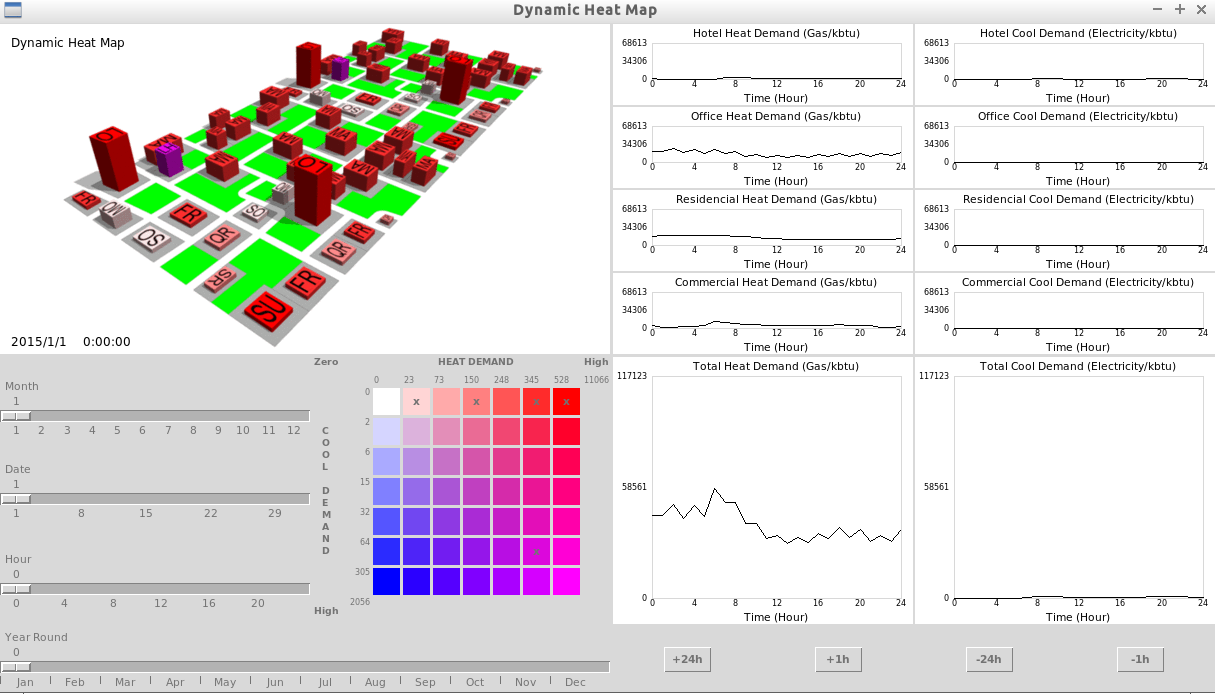
\includegraphics[width=0.7\linewidth]{interface0720}
  \caption{Dynamic Map Interface Layout (3D map)}
  \label{fig:interface0720}
\end{subfigure}
~
\begin{subfigure}
  \centering
  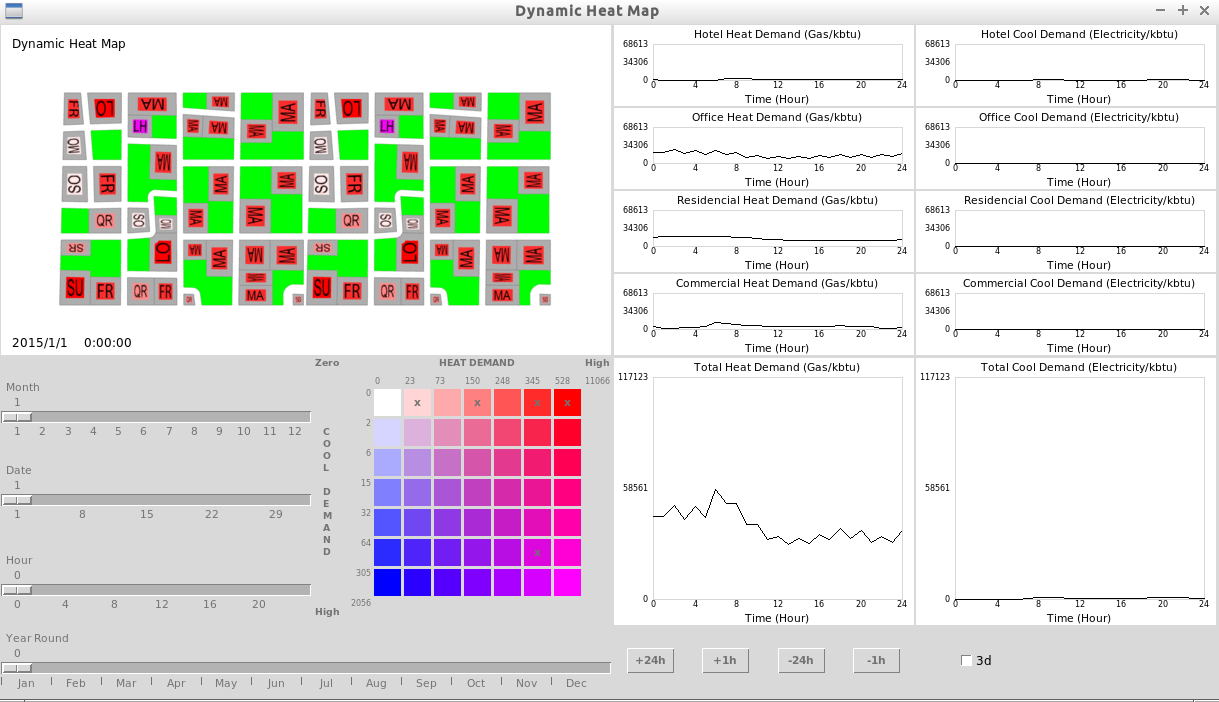
\includegraphics[width=0.7\linewidth]{interface2d}
  \caption{Dynamic Map Interface Layout (2D map)}
  \label{fig:interface2d}
\end{subfigure}
\caption{Dynamic Map Interface Layout}
\label{fig:interfaceLayout}
\end{figure}
Between the aggregated heat demand and the sliders, there is a
choropleth legend. According to section \ref{anime}, the comparison of
the map and the legend becomes tricky for dynamic maps. In order to
assist this task, tick marks of ``x'' are added to the legend to
indicate the color appeared in the map \fref{fig:legend}.
\begin{figure}[h!]
  \centering
  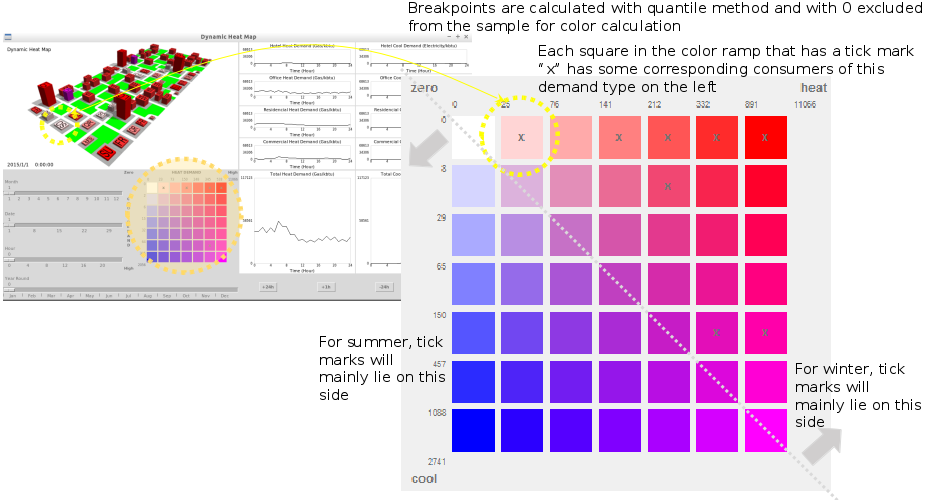
\includegraphics[width=0.7\linewidth]{legend}
  \caption{Bivariate Color Legend with Tick Mark Indicators}
  \label{fig:legend}
\end{figure}
\subsubsection {Navigation Function}
The navigation function is achieved with the four slider and the four
buttons above the sliders on the lower left of the window. The top
slider labeled with ``Year round'' has a range of 0 to 8760 (not
inclusive). the change of 1 in the slider position corresponds to the
change of 1 hour in time, which results in the display of the image of
the next or previous hour in time. The slider labeled with ``month''
has a range of 1 to 12, which corresponds to the 12 months in year,
the change of the month slider results the jump of 1 month forward or
backward in time. This function is intended to provide easy comparison
of montyly variation of the energy consumption behavior. Similarly,
the change of the ``date'' and ``hour'' slider corresponds to the time
change of one day or one hour respectively. The four buttons provides
a separate control intended to provide micro level adjustment of time.

\subsubsection {Dynamic Plot}
The input images to the main window is generated from the CityEngine
model. The graph is ploted by reading in simulation data from
EnergyPlus. The starting point (left end) of the plot corresponds to
the position indicated by the slider. 

\subsubsection {Implementation tools and strategy}
The softwares or platform involved in the project include EnergyPlus
for building simulation, CityEngine for 3D modeling and image
generation, Python 2.7 for interface design. The interface is written
in Python2.7 with standard Tkinter graphic package including the data
plot section.

\section{Case Analysis: Using the Current Dynamic Map to Design a District Energy System}
This section uses the tool assist the design of a district energy
network. The common steps in conducting such a design follows the
guidance of ~\cite{IDEA2012}. The goal of the case study is to
demonstrate how dynamic energy map can do better than static map in
assist the design of a district system and in demonstrating the
advantage of a district system. The major performance metric comparing
the static and dynamic map is the energy throughput.

As is suggested in the document~\cite{IDEA2012}, the data needed for
designing a district system include: 1) existing and emerging thermal
energy consumption, 2) fuel source availability and 3) land use
constraint. For the current case analysis on the conceptual setting,
the energy consumption is restricted to the heating gas energy
consumption and cooling electricity energy for the existing buildings.
The assumption about the central plant is it uses natural gas to
produce electricity, as is the most common case. It can also produce
chilled water with absorption chiller in summer. For land use
constraint, we assume the pipeline can be put only under the road
network.
 
\section{Findings and Discussion}
\subsection{Landuse Design on Load Balancing}

One of the point of having a visualization of dynamic map is, as
Dorling and Openshaw suggested, to detect mistakes that could
otherwise be neglected under a black box calculation routine or some
false application of rule of thumbs~\cite{Dorling1992}.

\grey{not finished}
\section{Conclusion}
  \begin{enumerate}[label*=\arabic*.]
  \item Summary of the current approach in implementing the dynamic
    Energy Map
  \item Limitations of the current implementation
    \begin{enumerate}[label*=\arabic*.]
    \item Simplified building simulation assumption about urban
      environment
    \item Lack of user choices for the stand-alone user interface as a
      result of its dependence on existing modeling softwares
    \end{enumerate}
  \item Future Expansion of the project
    \begin{enumerate}[label*=\arabic*.]
    \item Adding information of the supply side: residual energy,
      sustainable energy
    \item Providing different interfaces for different user population
    \item 2D and 3D compatible \\The reason for providing 2D map
      together with 3D map is that 2D maps have the following good
      properties:
      \begin{enumerate}[label*=\arabic*.]
      \item Better for region selection and spatial navigation than 3D
        map
      \item Better for conveying spatial relationship that does not
        involve height induced variation
      \item For larger scale display of city, state or nationwide, 3D
        building geometries becomes less significant in providing the
        urban environment context
      \end{enumerate}
    \item Creating an on-line tool for better information share
      \begin{enumerate}[label*=\arabic*.]
      \item Potential techniques: see 2.4
      \end{enumerate}
    \end{enumerate}
  \end{enumerate}
\item Acknowledgments
\end{enumerate}
\newpage

\begin{figure}[h]
  \centering
  \begin{subfigure}
  \centering
  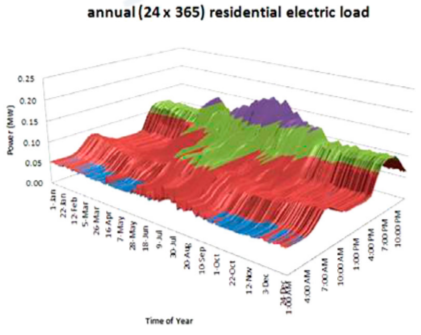
\includegraphics[width=0.4\linewidth]{resi}
  \caption{Residential Building Electricity Demand~\cite{baird2014}}
  \label{fig:resi}
\end{subfigure}
~
\begin{subfigure}
  \centering
  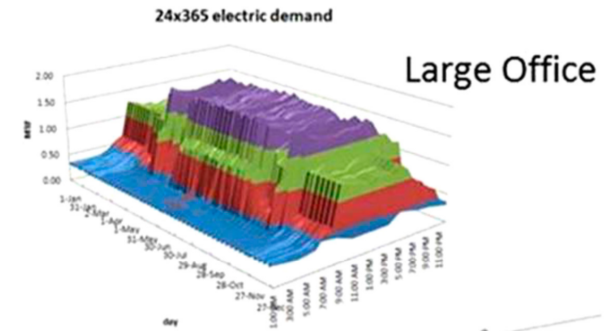
\includegraphics[width=0.4\linewidth]{office}
  \caption{Office Building Electricity Demand~\cite{baird2014}}
  \label{fig:office}
\end{subfigure}
\end{figure}

\begin{abstract}
  This document provides an approach of creating a space-time Energy
  Map, or a Dynamic Energy Map. The approach is demonstrated with a
  conceptual urban environment setting created in CityEngine based on
  the extracted topological and density pattern from an existing urban
  design project. The buildings in the conceptual model is then
  assigned an energy profile of certain DOE Commercial Benchmark
  Building Reference model based on its building type. Hourly energy
  heating and cooling demand profile are then obtained from the
  EnergyPlus simulation of DOE Commercial Benchmark models. The energy
  consumption data is classified into groups with consideration of
  \red{building energy design context} and the data distribution
  properties. A corresponding color coded energy profile is then
  generated and imported to CityEngine. 8760 color coded 2D and 3D map
  images was then extracted from CityEngine with Python script. A
  series of data reading, plotting, data classification and
  color-coding calculation utilities were implemented. An interactive
  interface for visualizing the images and dynamic data plot with
  sliders is implemented using Python. The tool is anticipated to
  provide decision insight for community energy management and
  planning, demand-side strategy design and district system sizing.
  
  The document will also briefly discuss one of the test-bed for data
  classification and visualization.

\end{abstract}
\end{comment}

\newpage
\bibliographystyle{plain}
\bibliography{myCitation}
\end{document}